\documentclass[11]{article}

\usepackage[inline]{enumitem}
\usepackage{graphicx}
\usepackage{gensymb}
\usepackage{float}

\usepackage{listings}
\usepackage{color}
\definecolor{darkgray}{rgb}{.35,.25,.35}
\definecolor{lightgray}{rgb}{.6,.6,.6}

\lstdefinelanguage{JavaScript}{
  keywords={typeof, new, true, false, catch, function, catch, switch, var, if, in, while, do, else, case, break},
  keywordstyle=\color{cyan}\bfseries,
  ndkeywords={return, null},
  ndkeywordstyle=\color{red}\bfseries,
  identifierstyle=\color{darkgray},
  sensitive=false,
  comment=[l]{//},
  morecomment=[s]{/*}{*/},
  commentstyle=\color{lightgray}\ttfamily,
  stringstyle=\color{red}\ttfamily,
  morestring=[b]',
  morestring=[b]"
}

\lstset{
   language=JavaScript,
   backgroundcolor=\color{white},
   extendedchars=true,
   basicstyle=\scriptsize\ttfamily,
   showstringspaces=false,
   showspaces=false,
   tabsize=2,
   breaklines=true,
   showtabs=false,
   captionpos=b
}

\title{
  Computational model for the Four Constraint Theory of human tool use\\  
  \setlength{\parskip}{0.5em}  
  \normalsize (PART 2 - Main Proposal)
  }
  
\date{}
\author{Adrian Ionita\\
\small{(NR: 1057404, ID: AFI904)}\\
Supervisor: Dietmar Heinke}

\hyphenation{thatshouldnot}

\begin{document}
\maketitle 	

The aim of this project is to develop a computational model for the four constraints theory(4CT).
4CT is not a complete definition of the psychological processes underlying tool use but a framework outlining cognitive components.   
The computational model will follow architecture considerations following 4CT.  As the theory lacks a complete description on mental processes involved, the model will have to make use of techniques outside of 4CT in order to produce more realistic examples of tool use . 

A computational model can not hope to capture all manner of tool use. The aim is to satisfy a specific set of problems, such as choosing the right tools for the desired tasks and breaking higher level objectives into intermediate steps.

\section{Test Driven Approach}

Test driven development is a common practice used in software development\cite{janzen2005}\cite{ibm2003}. It has a dual role of both testing the system and guiding development process\cite{janzen2005architecture}. When starting with a small set of tests that are subsequently satisfied, a system can incrementally grow to achieve increasingly complex solutions.The tests also naturally serve as an automatic way to ensure no damaging changes were introduced through the incremental process. The development of a computational model can benefit from the same tight feedback process.

A model prerequisite is therefore to determine a set of tests that will prove its validity. As the theory is based on investigations of apraxia patients, a good set of tests should be based on this research. In the last 20 years, experiments have been split between pantomime of tool use (i.e. miming), single tool use, real tool use and mechanical problem solving\cite{baumard2014}. Because of the focus on technical reasoning, the latter two are most suitable in the context of 4CT. The implementation will start with the simplest tests to satisfy and move to more complex ones as it progresses.

\subsection{Real Tool Use Experiments}

In real tool use tasks, subjects are required to select an appropriate tool to act on a given object\cite{baumard2014}. The experiments can have multiple tools or target objects serving as distractors. These tasks can grow in complexity by requiring multiple sequences of actions to satisfy an objective.

Tests for this type of scenario will simply involve a categorical matching of objects. For example, if our goal is to have a slice of bread we will choose a knife instead of a saw for cutting. This is because the bread and the knife are semantically kitchen items. At the same time, when choosing between a fork and a knife, we would choose the item which semantically is known to be a cutting device. 

The experimental inputs will be an arbitrary sets of objects: hammer, knife, bread, walnut etc. Accompanying them, will be an objective (e.g. getting a slice a of bread). The model should be able to determine the optimal item combination to satisfying the objective. 

\subsection{Mechanical Problem Solving}

Mechanical problem solving experiments are similar to real tool use tasks. The difference is that these involve novel uses of tools and objects(e.g. screwing a screw with a knife\cite{baumard2014} or using a stone to hammer\cite{zhu2015}). 

Single tool to object matching will prove simple when fitting is done based on the object's physical properties. For example, if no hammer is available, a rock's weight and hardness would suffice in cracking a nut. 4CT gives convincing examples of how this matching can work. 

Later tests can focus on geometric fitting of objects or on how higher level goals are split into sub-goals and tasks. Although geometric consideration will be more convincing, they will, however, not enable testing of other components of the theory, such as working memory and simulation based decision making. An appropriate choice of tests will depend on the time that is available. 

\section{Symbolic Model}

4CT does not concentrate on the neural basis for tool use, with considerations taken only on brain areas involved in this ability. The focus is on high level mental structures. As such, a good starting point for a computational model is one of a symbolic nature (i.e. symbolic AI), instead of a neurally feasible implementation (i.e. connectionist AI)\cite{smolensky87}. Below we outline the responsibilities, within the model, of each of the 4CT components. The way these components interact with each other will become apparent during model implementation.

\subsection{Technical Reasoning}

Technical reasoning is based on object based knowledge (e.g. hardness, length, abrasiveness) and mechanical knowledge (i.e. how tool movement transforms into physical principles)\cite{osiurak2014}.

4CT suggests a distinction between tools and objects.  Since objects can become novel tools, a better implementation would completely ignore this difference. Therefore, a tool is any object that can be handled to form environment transformations. 

In terms of representation, objects can be seen as multidimensional structures represented through their physical properties. This is equivalent to 4CT's notion of object knowledge. These dimensions are continuous in value, rather than discrete. 

Mechanical knowledge will be tied to the technique of use (e.g. poking, cutting, hitting). In terms of representation, they can be seen as functions that would create additional dimensions on the object's representation. For example, a lever property would generate a lever force with a certain precision of control. These dynamic properties are dependent on physical aspects of the object (i.e. length , weight ) and on the mode of usage (i.e. grip location and applied force). Below (fig.\ref{fig:hammer}), is an illustration of how different tool use parameters generates new dimensions. 
\begin{figure}[h]
\centering
\begin{tabular}{p{0.40\textwidth} p{0.60\textwidth}}
  \vspace{0pt} 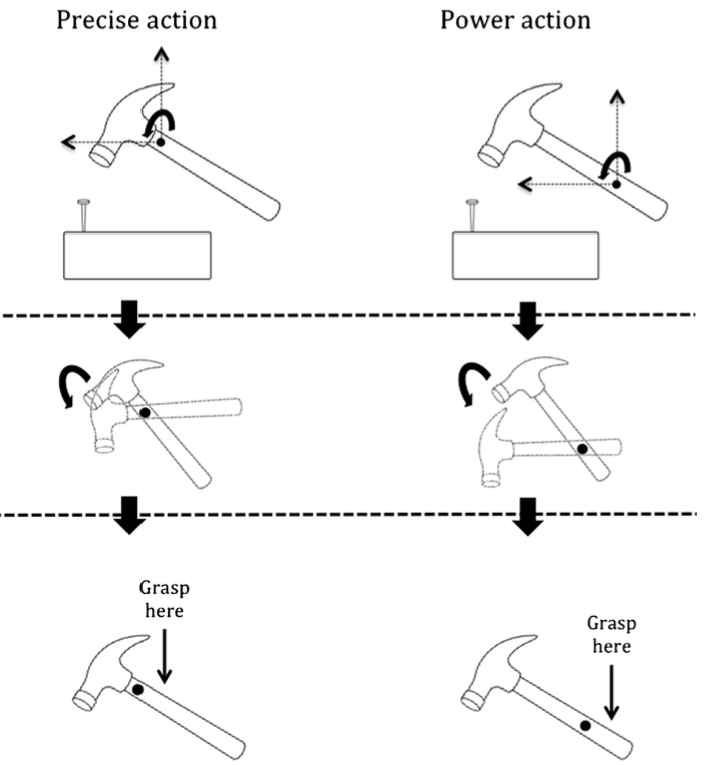
\includegraphics[width=0.45\textwidth]{hammering.png} &
  \vspace{0pt} \begin{lstlisting}
//hammer struct
 { 
	length   : 10
	hardness : 20 
	weight   : 20 
	leaver: function(appliedForce,gripLocation)
	{
		var leverForce = (appliedForce+weight) *  gripLocation/(length-gripLocation);
		
		var precission = 1 / leverForce;

		return [leverForce,precission];
	}
 }
  \end{lstlisting}
\end{tabular}
  
      \caption{  
   Figure taken from \cite{osiurak2014}
   }
   \label{fig:hammer}

\end{figure}

The above notions are sufficient to test the technical reasoning aspects of 4CT. They follow closely the examples given within the theory's paper. The notions are particularly useful in tool use experiments such as tool to object matching (fig. \ref{fig:knife}).

\begin{figure}[h]
	\label{fig:knife}
	\centering
	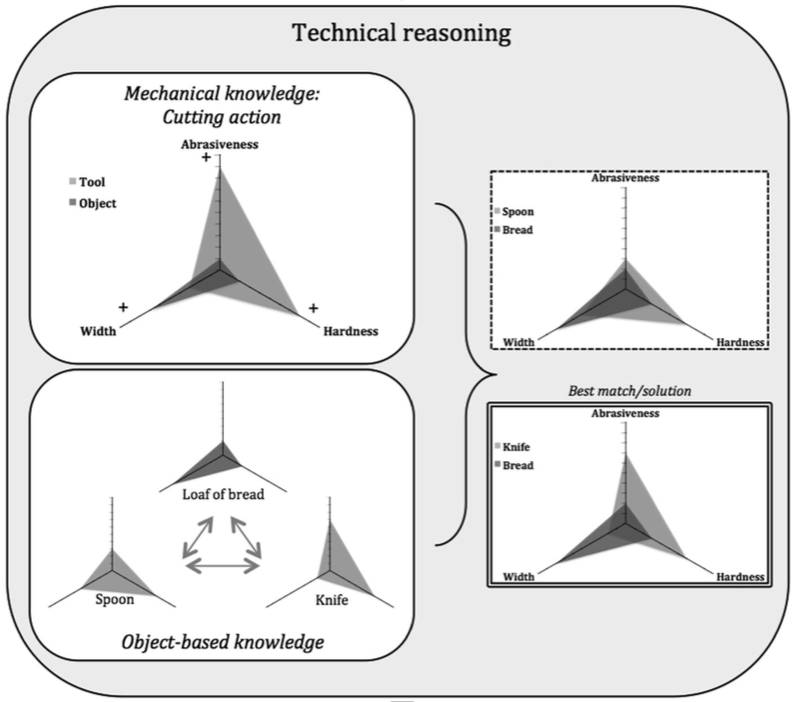
\includegraphics[width=1\textwidth]{knife.png}
	\caption { Figure taken from \cite{osiurak2014} }
\end{figure}

It becomes difficult to conceptualise what happens when the object's shape and contact surface are involved. When working with geometric shapes, each pixel or voxel, can be seen as a feature in representing the object. Tool to object matching may still function on such multidimensional fitting, but the scalability of the approach is uncertain. For example, would the blade of a knife emerge conceptually from independent voxels  when cutting? Can the voxels of the tip of the knife fit algorithmically the head of a screw to turn it? Geometric fitting outside of 4CT specifications will have to be used.

The disadvantage of a symbolic approach is the necessity to manually choose parameters of the objects. A more credible implementation is one which infers properties based on observation such as in \cite{zhu2015}. It is uncertain however, the level of complexity of the tasks that can be learnt from observations ( e.g. can we learn writing from just observation ). If time allows for advancements, the  model will consider training neural networks for detecting object properties.

\subsection{Semantic Reasoning}

Semantic reasoning serves as a shortcut for selecting appropriate tools. Real tool use experiments, exercise semantic reasoning more than mechanical reasoning. Selecting an appropriate tool involves consideration of the tool's functionality rather than physical properties. This is in contrast to technical reasoning but the two processes work tightly together. 


\subsection{Working Memory}

4CT presents working memory in the context of tool use tasks requiring multiple steps. For example, making a jam sandwich requires locating the ingredients, slicing a loaf of bread and finally spreading jam over a slice\cite{osiurak2014}. 

The author makes predictions on the effects of impairing memory with either time or storage constraints\cite{osiurak2014}. The difficult aspect, however, is how subjects are able to split higher level objectives into sub-goals to begin with. 4CT does not elude to this process, which adds risk to a successful implementation in this area. 

\subsection{Mental Simulation}

Simulation decision making will help select an optimal tool based on its estimated required effort of use. This will be measured based on the tool's fitness to the task, where unfit tools will be considered to require more effort than those with correct property values. Additionally we may consider the subject's experience with the technique of use, although this is not covered by 4CT.

\section{Neural Feasibility}
It would prove interesting to see if neural networks can be trained to capture object properties. Multiple trained networks could work in conjunction to represent the multidimensional properties of tools. The way these representations can interact or if they can be trained from experience is generally unexplored. A neurally feasible approach is a secondary concern to this project. The approach would be tackled only if time is available and starting with capturing object physical properties. 


\begin{thebibliography}{9}

\bibitem{janzen2005}
Janzen, D., \& Saiedian, H. (2005). \emph{Test-driven development concepts, taxonomy, and future direction}. Computer, 38(9), 43–50. doi:10.1109/mc.2005.314

\bibitem{ibm2003}
Maximilien, E. M., \& Williams, L. (2003). \emph{Assessing test-driven development at IBM}. 25th International Conference on Software Engineering, 2003. Proceedings. doi:10.1109/icse.2003.1201238

\bibitem{janzen2005architecture}
Janzen, D. S. (2005). \emph{Software architecture improvement through test-driven development}. Companion to the 20th annual ACM SIGPLAN conference on Object-oriented programming, systems, languages, and applications - OOPSLA ’05. doi:10.1145/1094855.1094954

\bibitem{smolensky87}
Smolensky, P. (1987). \emph{Connectionist AI, symbolic AI, and the brain}. Artificial Intelligence Review, 1(2), 95–109. doi:10.1007/bf00130011

\bibitem{osiurak2014}
Osiurak, F. (2014). \emph{What Neuropsychology tells us about human tool use? The Four constraints theory (4CT): Mechanics, space, time, and effort}. Neuropsychology Review, 24(2), 115 - 88. doi:10.1007/s11065-014-9260-y

\bibitem{baumard2014}
Baumard, J., Osiurak, F., Lesourd, M., \& Le Gall, D. (2014). \emph{Tool use disorders after left brain damage}. Frontiers in Psychology, 5, . doi:10.3389/fpsyg.2014.00473


\bibitem{zhu2015}
Zhu, Y., Zhao, Y., \& Zhu, S.-C. (2015). \emph{Understanding tools: Task-oriented object modeling, learning and recognition}. 2015 IEEE Conference on Computer Vision and Pattern Recognition (CVPR). doi:10.1109/cvpr.2015.7298903



\end{thebibliography}


\end{document}